This section offers some basic conclusion in  Teichm\"uller theory and hyperbolic geometry. Details can be found in \cite{Imayoshi1992An} and \cite{Buser}.

Fix $S$ to  be  an oriented  connected closed surface. The Teichm\"uller space $\mathscr{T}(S)$ contains the equivalent classes of $(X,f)$, where $X$ is a complete hyperbolic surface, and $f \colon S\to X$ is a diffeomorphism, which is said to define a marking on $X$. $(X,f)$ and $(Y,g)$ are equivalent if $f\circ g^{-1} \colon Y\to X$ is isotopic to a conformal map. 

If $\partial S$ is not empty, set $A$ to be all connecting components for $\partial S$, and set $L=(L_\alpha)_{\alpha\in A}$ with $L_\alpha>0$. Then a point $(X,f)$ in $\mathscr{T}(S,L)$  is a diffeomorphism $f \colon S\to X$ of $S$ onto a hyperbolic surface with geodesic boundary components of fixed length,
$$l_{\alpha}(X)=L_\alpha.$$ 

Notice that there may exist a conformal automorphism  $f \colon X\to X$ which is not isotopic to the identity map.
 
For  $S=S_{g,n}$, the surface of genus $g$ with $n$  boundary components, set 
$$
\mathscr{T}_{g,n}(L)=\mathscr{T}(S_{g,n},L).
$$
For $3g-3+n>0$, $\mathscr{T}_{g,n}(L)$ is of real dimension $6g-6+2n$.

Define 
$$\Mod(S)=\diff(S)/\diff_0(S)$$ 
to be  the mapping class group of $S$.  Here $\diff(S)$ is the group of  orientation preserving self diffeomorphisms which  map each boundary component to itself as a set,  and $\diff_0(S)$ is the group of  orientation preserving self diffeomorphisms which is isotopic to the identity map.

Set $\Mod_{g,n}=\Mod(S_{g,n})$, and it acts on $\mathscr{T}_{g,n}(L)$ as 
$$
\begin{aligned}
    \Mod_{g,n}\times \mathscr{T}_{g,n}(L)&\to \mathscr{T}_{g,n}(L)\\
    h\circ  (X,f)&\mapsto (X,f\circ h^{-1}).\\
\end{aligned}
$$
Then it induces the  quotient space $$
\mathscr{M}(S_{g,n},L)=\mathscr{M}_{g,n}(L) =\mathscr{T}_{g,n}(L)/\Mod_{g,n},
$$
called the moduli space  of Riemann surface homeomorphic to $S_{g,n}$  with fixed  boundary length $L$.

If $L_\alpha=0$, then the geodesic boundary component corresponds to $\alpha$ is a cusp,  which will be described in section \ref{MMid}. Define $\mathscr{T}_{g,n}=\mathscr{T}_{g,n}(0,0,\cdots,0)$ and $\mathscr{M}_{g,n}=\mathscr{M}_{g,n}(0,0,\cdots,0)$.


If $S$ is not connected, write it as $S=\cup_iS_i$ with $S_i$ 
connected, then define $$\mathscr{M}(S,L)=\prod_{i}\mathscr{M}(S_i,L_{\partial S_i}).$$

For $S_{g,n}$ with $3g-3+n>0$, any $3g-3+n$ non-trivial disjoint simple closed geodesics will cut $S_{g,n}$ into $2g-2+n$ pairs of pants, or $S_{0,3}$. The details will be showed in section \ref{hypergeo}.  Call such a system of closed geodesics which  cuts $S_{g,n}$ into pants  a pants decomposition. Denote them by $P=\{\alpha_i\}_{i=1}^{3g-3+n}.$ For $\alpha_i$ and $(X,f)\in \mathscr{T}_{g,n}(L),$ $f(\alpha_i)$ is a non-trivial simple closed curve, but may not be a geodesic. Among the homotopy class $[f(\alpha_i)]$, there is  a unique geodesic $\tilde{\alpha_i}$ which is of minimal length, and denote the length of it  by $l_{\alpha_i}(X).$ The shortest geodesic can be approximated by taking the length-minimal sequence.

For two pairs of pants adjoint to $\tilde{\alpha_i}$, fix two marking points,  the directed length $\tau_{\alpha_i}(X)$ between them along $\tilde{\alpha_i}$ can parameterize how they are glued along $\tilde{\alpha_i}$. $\tau_{\alpha_i}(X)$ is called the twisting parameter of $X$ along $\alpha_i$.

Fix the pants decomposition $P=\{\alpha_i\}_{i=1}^{3g-3+n}$, $(X,f)\in \mathscr{T}_{g,n}(L)$ can be parameterized by the Fenchel-Nielsen coordinates with respect to $P$, $$(l_{\alpha_1}(X),\cdots,l_{\alpha_k}(X),\tau_{\alpha_1}(X),\cdots,\tau_{\alpha_k}(X)).$$
The map $$
\begin{aligned}
\mathscr{T}_{g,n}(L)&\to \mathbb{R}_{+}^{P}\times\mathbb{R}^{P}\\
(X,f)&\to (l_{\alpha_i}(X),\tau_{\alpha_i}(X))\\
\end{aligned}
$$
 is an isomorphism.
 
There is a basic fact in hyperbolic geometry called the Collar Lemma. 

\begin{lemma}[Collar Lemma]\label{collarlemma}
  For a simple closed geodesic $\gamma$ in $S_{g,n}$ with length $l(\gamma)$, define  the collar  $T(\gamma)$ with center geodesic $\gamma$ to be the domain  
  $$
  \{x\in S_{g,n}|d(x,\gamma)\leq w(\gamma)\},
  $$
  where $w(\gamma)=\operatorname{arcsinh}\frac{1}{\operatorname{sinh}{\frac{1}{2}l(\gamma)}}$ is the half width of the collar.
  Then $T(\gamma)$ is isomorphic to a cylinder parameterized by $[-w(\gamma),w(\gamma)]\times (\mathbb{R}/\mathbb{Z})$,  with the metric 
$$ ds^2=d\rho^2+l(\gamma)^2\cosh^2\rho dt^2.
$$
Here  $\rho$ represents the directed distance from $\gamma$, and $t$ parameterizes the projection point on $\gamma$.
For two disjoint  simple closed geodesics $\gamma_1$ and $\gamma_2$, the corresponding collars $T(\gamma_1)$ and $T(\gamma_2)$ are disjoint.

\end{lemma}

\begin{figure}[h]
    \centering
    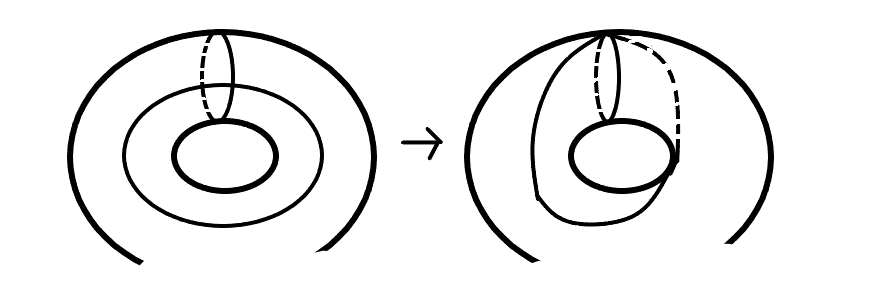
\includegraphics[width=4 in]{picture/dehntwist.png}
    \caption{Dehn twist}
    \label{fig:dehntwist}
\end{figure}

Along $\gamma\subset S_{g,n}$, there is a self-homeomorphism $D_{\gamma}$ which is invariant outside the collar $T(\gamma)$, and is not homotopic to the identity map.  In the coordinate representation, $$
 D(\gamma) \colon (\rho,t)\mapsto (\rho, t+\frac{\rho+w(\gamma)}{2w(\gamma)}).
 $$
 $D(\gamma)$ is not smooth, but is homotopic to a smooth self-diffeomorphism $\phi_\gamma$ of $S_{g,n}$, which is a non-trivial element in $\Mod_{g,n}(L)$, called the Dehn twist along $\gamma$.See figure \ref{fig:dehntwist}.
 
 \begin{figure}[h]
    \centering
    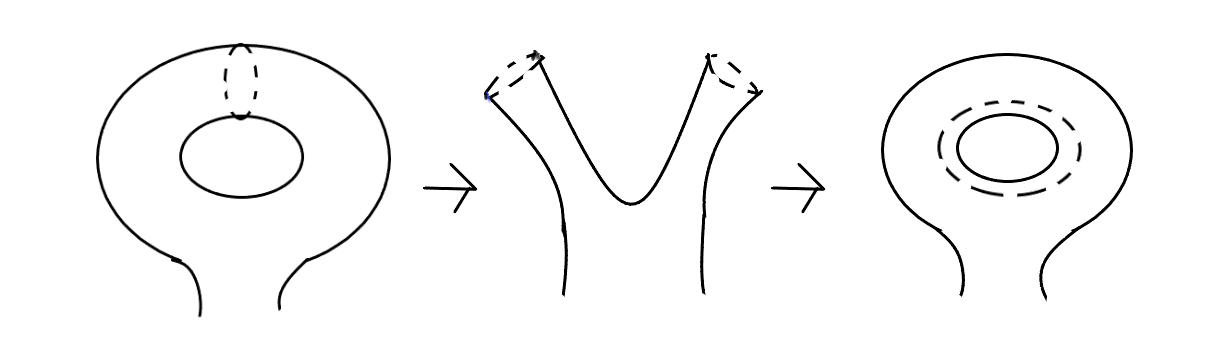
\includegraphics[width=5 in]{picture/halftwist.png}
    \caption{Half twist}
    \label{fig:halftwist}
\end{figure}

For $S_{1,1}$, there is a half twist  $\sigma$ of order two belonging to $\Mod_{1,1}(L)$ shown as the Figure \ref{fig:halftwist}. $\sigma$ maps  $a$-circle to $b$-circle, and maps $b$-circle to the inversion of  $a$-circle. 

For a given pants decomposition $P$, the mapping class group $\Mod_{g,n}(L)$ acts on $\mathscr{T}_{g,n}(L)$ by the components of Dehn twists long the pants decomposition $P$ and half twists on  $S_{1,1}$ parts cut by some simple closed geodesic $\alpha_i$ belong to the pants decomposition.  

 
 
 $\mathscr{T}_{g,n}(L)$ has a symplectic structure, and the symplectic form $\omega\in \Omega^2(\mathscr{T}_{g,n}(L))$ is invariant under the $\Mod_{g,n}(L)$ action. It is called Weil--Petersson symplectic form, and induces a volume form $$
 \frac{1}{(3g-3+n)!}\wedge^{3g-3+n}\omega
 $$
 on $\mathscr{T}_{g,n}(L)$, called Weil--Petersson volume form, which is also invariant under $\Mod_{g,n}(L)$ action, hence both the Weil--Petersson symplectic form and Weil--Petersson volume form can degenerate  to $\mathscr{M}_{g,n}(L)$.
 
 Wolpert represent the Weil--Petersson symplectic form  by the Fenchel-Nielsen coordinates \cite{wolpertformula}.
 \begin{theorem}\label{wpmetricWolpert}
 The Weil-Petersson symplectic form is 
 $$
 \omega=\sum_{i=1}^{3g-3+n}dl_{\alpha_i}\wedge d\tau_{\alpha_i},
 $$ under Fenchel-Nielsen coordinates $(l_{\alpha_i},\tau_{\alpha_i})$.
 \end{theorem}
 
\begin{remark}
The fact that Weil-Petersson form is a symplectic form, or a non-degenerated closed form can be  directly  seen from this representation. 
The Dehn twist $\phi_{\alpha_i}$ along $\alpha_i$ acts on $\mathscr{T}_{g,n}(L)$ by 
$$
(l_{\alpha_j},\tau_{\alpha_j})_{j=1}^{3g-3+n}\mapsto
(l_{\alpha_j},\tau_{\alpha_J}+\delta_{ij}l_{\alpha_j})_{j=1}^{3g-3+n},
$$
where $\{\alpha_{j}\}_{j=1}^{3g-3+n}$ is a pants decomposition containing $\alpha_i$.
Therefore $\omega$ is invariant under $\Mod_{g,n}(L)$.
\end{remark}

For $S_{g,n}$ with $L\in \mathbb{R}_+^{3g-3+n}$, define $\mathrm{Vol}(\mathscr{M}(S,L))$ to be the Weil--Petersson volume of the moduli space $\mathscr{M}_{g,n}(L)$,  and for the disconnected surface $S=\cup_{i}S_i$, the Weil--Petersson volume is $$
\mathrm{Vol}(\mathscr{M}(S,L))=\prod_{i}\mathrm{Vol}(\mathscr{M}(S_i,L_{S_i})).
$$





